\subsection{Controls}
The controls for the game are presented in the \autoref{tab:game_key_functions}.
If the user forgets them they can at any time press the "Controls" button in the menu to see them in game as shown in Figure \ref{fig:controls}.

\begin{table}[h]
    \centering
    \begin{tabular}{|m{3cm}|m{8cm}|}
    \hline
    \textbf{Key} & \textbf{Function} \\
    \hline
    \texttt{W} & Move Forward \\
    \hline
    \texttt{S} & Move Back \\
    \hline
    \texttt{A} & Move Left \\
    \hline
    \texttt{D} & Move Right \\
    \hline
    \texttt{Shift} & Sprint \\
    \hline
    \texttt{Space} & Jump \\
    \hline
    \texttt{Left Mouse} & Use Item \\
    \hline
    \texttt{Right Mouse} & Use Item's second ability \\
    \hline
    \texttt{Esc} & Show/Hide Menu \\
    \hline
    \texttt{Tab} & Switch Camera between 1st and 3rd person \\
    \hline
    \texttt{Scroll} & Change FOV \\
    \hline
    \texttt{0-9} & Select Item \\
    \hline
    \texttt{C} & Enter Car \\
    \hline
    \texttt{F} & Flip Car (only works outside the car) \\
    \hline
    \texttt{L} & Leave Car \\
    \hline
    \texttt{Y} & Toggle Flashlight/Toggle car reflectors (when inside the car) \\
    \hline
    \end{tabular}
    \caption{Keyboard Key Functions for Game Controls}
    \label{tab:game_key_functions}
\end{table}

\begin{figure}[H]
    \centering
    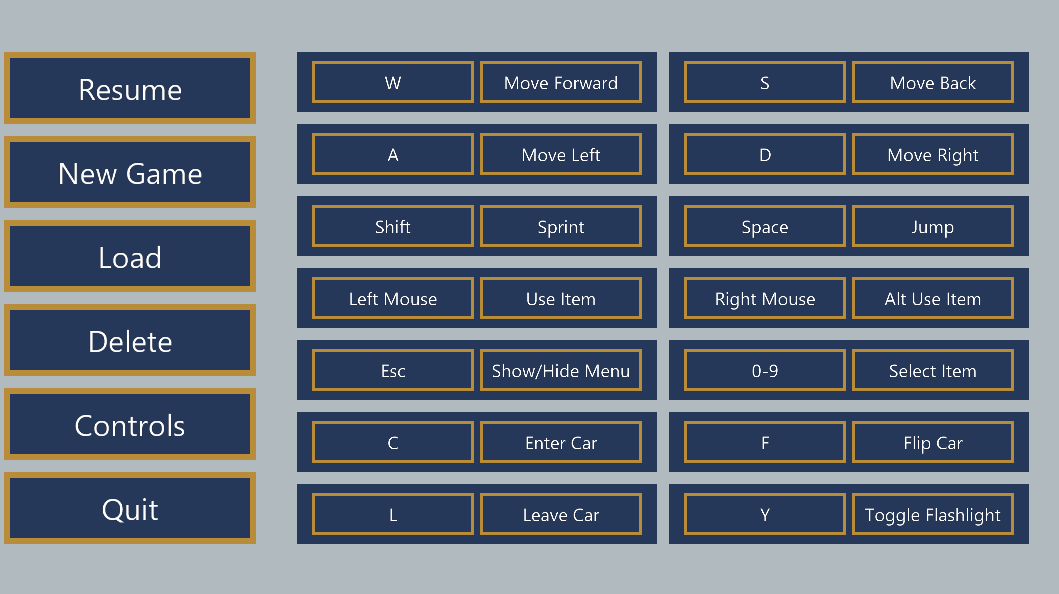
\includegraphics[width=0.8\textwidth]{sections/user_manual/resources/controls.png}
    \caption{Controls screen}
    \label{fig:controls}
\end{figure}